%% Do not edit preable unless you know what you are doing.
\documentclass{article}\usepackage[]{graphicx}\usepackage[]{color}
% maxwidth is the original width if it is less than linewidth
% otherwise use linewidth (to make sure the graphics do not exceed the margin)
\makeatletter
\def\maxwidth{ %
  \ifdim\Gin@nat@width>\linewidth
    \linewidth
  \else
    \Gin@nat@width
  \fi
}
\makeatother

\definecolor{fgcolor}{rgb}{0.345, 0.345, 0.345}
\newcommand{\hlnum}[1]{\textcolor[rgb]{0.686,0.059,0.569}{#1}}%
\newcommand{\hlstr}[1]{\textcolor[rgb]{0.192,0.494,0.8}{#1}}%
\newcommand{\hlcom}[1]{\textcolor[rgb]{0.678,0.584,0.686}{\textit{#1}}}%
\newcommand{\hlopt}[1]{\textcolor[rgb]{0,0,0}{#1}}%
\newcommand{\hlstd}[1]{\textcolor[rgb]{0.345,0.345,0.345}{#1}}%
\newcommand{\hlkwa}[1]{\textcolor[rgb]{0.161,0.373,0.58}{\textbf{#1}}}%
\newcommand{\hlkwb}[1]{\textcolor[rgb]{0.69,0.353,0.396}{#1}}%
\newcommand{\hlkwc}[1]{\textcolor[rgb]{0.333,0.667,0.333}{#1}}%
\newcommand{\hlkwd}[1]{\textcolor[rgb]{0.737,0.353,0.396}{\textbf{#1}}}%
\let\hlipl\hlkwb

\usepackage{framed}
\makeatletter
\newenvironment{kframe}{%
 \def\at@end@of@kframe{}%
 \ifinner\ifhmode%
  \def\at@end@of@kframe{\end{minipage}}%
  \begin{minipage}{\columnwidth}%
 \fi\fi%
 \def\FrameCommand##1{\hskip\@totalleftmargin \hskip-\fboxsep
 \colorbox{shadecolor}{##1}\hskip-\fboxsep
     % There is no \\@totalrightmargin, so:
     \hskip-\linewidth \hskip-\@totalleftmargin \hskip\columnwidth}%
 \MakeFramed {\advance\hsize-\width
   \@totalleftmargin\z@ \linewidth\hsize
   \@setminipage}}%
 {\par\unskip\endMakeFramed%
 \at@end@of@kframe}
\makeatother

\definecolor{shadecolor}{rgb}{.97, .97, .97}
\definecolor{messagecolor}{rgb}{0, 0, 0}
\definecolor{warningcolor}{rgb}{1, 0, 1}
\definecolor{errorcolor}{rgb}{1, 0, 0}
\newenvironment{knitrout}{}{} % an empty environment to be redefined in TeX

\usepackage{alltt}
\usepackage[sc]{mathpazo}
\usepackage[T1]{fontenc}
\usepackage[english]{babel}
\usepackage[utf8]{inputenc}
\usepackage{geometry}
\usepackage{dsfont}
\usepackage{indentfirst}
\usepackage{fancyhdr}
\usepackage{amsmath}
\usepackage{enumitem}

% No indents in whole document
\setlength\parindent{0pt}

% Gaps between item is itemize
\setitemize{itemsep=-1em,topsep=0.5em,parsep=0em,partopsep=0pt}

% Margins of the document
\geometry{verbose,tmargin=2.5cm,bmargin=2.5cm,lmargin=2.5cm,rmargin=2.5cm}

% Header and footer for all pages
\pagestyle{fancy}
\fancyhf{}
\renewcommand{\headrulewidth}{0pt}
\rfoot{Page \thepage}

% Header and footer for first page
\fancypagestyle{plain}{%
  \renewcommand{\headrulewidth}{0pt}%
  \fancyhf{}%
  \rhead{ETH Zurich}
  \lhead{Applied Generalized Linear Models \\ Spring Semester 2020}
  \rfoot{Page \thepage}
}

% Global Settings of R-code


% Mathematics Operators for Ease of Notation
\DeclareMathOperator{\SSR}{SSR}
\DeclareMathOperator{\SSreg}{SSreg}
\DeclareMathOperator{\SST}{SST}

% Bad Box settings
\hbadness=10000
\vbadness=\maxdimen
\vfuzz=30pt
\hfuzz=30pt


%% ---------- BEGIN DOCUMENT -----------------------------------------------
\IfFileExists{upquote.sty}{\usepackage{upquote}}{}
\begin{document}

%% Tiltle
\title{Assignment 1}
\author{Milan Kuzmanovic, Mark McMahon \\ Martin Kotuliak, Jakub Polak}
\date{\today}
\maketitle

\section*{Task 1}

A multiple linear regression model has been estimated to study the relationship between $Y =$ violent crime rate (per 100,000 people), $X_1 =$ poverty rate (percentage with income below the poverty line) and $X_2 =$ percentage living in urban area. Data are collected in 51 cities in the U.S.\\

The relevant equations that relate estimates, standard error, T-statistic, R-squared and Sum of Squares of residuals, regression, and total are the following.

\[ \frac{\beta_i}{se(\beta_i)} = T_i \qquad R^2 = \frac{\SSreg}{\SST}= 1-\frac{\SSR}{\SST}  \qquad \SST = \SSreg + \SSR
\]

We plug in the corresponding information that is already provided and compute the missing values.

\begin{knitrout}
\definecolor{shadecolor}{rgb}{0.969, 0.969, 0.969}\color{fgcolor}\begin{kframe}
\begin{alltt}
\hlstd{a} \hlkwb{<-} \hlopt{-}\hlnum{498.683} \hlopt{/} \hlnum{140.988}
\hlstd{b} \hlkwb{<-} \hlnum{4.885} \hlopt{*} \hlnum{6.677}
\hlstd{c} \hlkwb{<-} \hlnum{9.112} \hlopt{/} \hlnum{6.900}
\hlstd{d} \hlkwb{<-} \hlnum{1841257.15} \hlopt{/} \hlstd{(}\hlnum{1} \hlopt{-} \hlnum{0.5708}\hlstd{)}
\hlstd{e} \hlkwb{<-} \hlstd{d} \hlopt{-} \hlnum{1841257.15}
\end{alltt}
\end{kframe}
\end{knitrout}

The table below reports the output with filled in missing information.

\begin{center}
\begin{tabular}{ l r r r r }
 \hline
            & Est.            & s.e.              & t-value         & p-value \\
 \hline
 Intercept  & -498.683  & 140.988 & $^{a\;}$-3.537 & 0.009 \\
 $X_1$      & $^{b\;}$32.617 & 6.677  & 4.885     & 0.001 \\
 $X_2$      & 9.112  & $^{c\;}$1.321 & 6.900      & 0.001 \\
 \hline
 $R^2$      & 0.5708            & & & \\
 SSreg      & $^{e\;}$2448717.57 & & & \\
 SSR        & 1841257.15        & & & \\
 SSTotal    & $^{d\;}$4289974.72 & & & \\
 \hline
\end{tabular}
\end{center}

The coefficient of determination $R^2$ is $0.5708$. This value measures the proportion of the variance in $Y$ explained by the model. Hence, 57.08 \% of the sample variability of $Y$ can be explained by the linear combination of $X_i$'s given the sample data. \\

To compute the overall F-test we use the equation below and the statistic then follows an F distribution with corresponding degrees of freedom.
\[ F = \frac{\SSreg/p}{\SSR/(n-(p+1))} \sim F_{p,n-(p+1)}
\]

The data are collected in 51 cities, so $n=51$ and we have 2 predictors, so $p=2$. Other values we can easily obtain from the filled table above.
\begin{knitrout}
\definecolor{shadecolor}{rgb}{0.969, 0.969, 0.969}\color{fgcolor}\begin{kframe}
\begin{alltt}
\hlstd{(f} \hlkwb{=} \hlstd{(e} \hlopt{/} \hlnum{2}\hlstd{)} \hlopt{/} \hlstd{(}\hlnum{1841257.15} \hlopt{/} \hlstd{(}\hlnum{51}\hlopt{-}\hlstd{(}\hlnum{2}\hlopt{+}\hlnum{1}\hlstd{)) ))}
\end{alltt}
\begin{verbatim}
## [1] 31.91799
\end{verbatim}
\end{kframe}
\end{knitrout}

Hence, the F-statistic has a value of 31.917987. To interpret this, the global F-test tests a null hypothesis that all regression coefficients are simultaneously 0. In a mathematical notation $H_0 : \beta_1 = \beta_2 = 0$. To evaluate the test, we can compute its p-value. It is a quantile of the corresponding F-distribution for the given statistic or mass under the distribution.

\begin{knitrout}
\definecolor{shadecolor}{rgb}{0.969, 0.969, 0.969}\color{fgcolor}\begin{kframe}
\begin{alltt}
\hlstd{(p} \hlkwb{=} \hlkwd{pf}\hlstd{(f,}\hlnum{2}\hlstd{,}\hlnum{48}\hlstd{,}\hlkwc{lower.tail} \hlstd{=} \hlnum{FALSE}\hlstd{))}
\end{alltt}
\begin{verbatim}
## [1] 1.526979e-09
\end{verbatim}
\end{kframe}
\end{knitrout}

The p-value is \ensuremath{1.5269792\times 10^{-9}}, which is lower than the significance level $\alpha=0.05$ and therefore, there is a significant evidence against the null hypothesis that all regression coefficients are simultaneously zero. Hence, the p-value of a given sample is small and it suggests that the model with all the covariates is better than the one with just intercept coefficient. This test determines the linear model is suitable to explain some of the variance in the outcome variable. Which in this case it does.

\section*{Task 2}

The table below shows the scores of the first test (maximum score 10 points) in a beginning German course. Students in the course are grouped as follows:
\begin{itemize}
\item Group A: Never studied foreign language before, but have good English skills\\
\item Group B: Never studied foreign language before, have poor English skills\\
\item Group C: Studied other foreign language
\end{itemize}

\begin{center}
\begin{tabular}{ c c c }
 \hline
 Group A & Group B & Group C \\
 \hline
 4 & 1 & 9 \\
 6 & 5 & 10 \\
 8 &   & 5 \\
 \hline
\end{tabular}
\end{center}

Two-sample t-test is an often used method for comparing mean scores of two groups. The one-way analysis of variance (ANOVA), also known as one-factor ANOVA, is an extension of independent two-samples t-test for comparing means in a situation where there are more than two groups. This corresponds to our situation.\\

The Hypothesis test in ANOVA is following:
\begin{itemize}
\item Null hypothesis: the means of the different groups are the same; \\
\item Alternative hypothesis: At least one sample mean is not equal to the others.
\end{itemize}

The Assumptions of ANOVA are following:
\begin{itemize}
\item The observations are obtained independently and randomly from the population defined by the groups of factor levels;\\
\item The data of each factor level are normally distributed;\\
\item These normal populations have a common variance.
\end{itemize}

The F-test is used for comparing the factors of the total deviation. In ANOVA, the F-statistic is computed as the ratio of the variance between groups and variance within groups. The F-statistic is then compared to the F-distribution with $I-1$ and $n-I$ degrees of freedom, where $I =$ total number of groups and $n =$ total number of observations. Note that, a lower ratio (ratio $< 1$) indicates that there are no significant difference between the means of the samples being compared. However, a higher ratio implies that the variation among group means are significant.\\

The process of ANOVA testing is following:
\begin{itemize}
\item Compute the common variance, which is called variance within samples $S^2_{\text{within}}$ or residual variance.\\
\item Compute the variance between sample means, by first computing the mean of each group and then computing the variance between sample means $S^2_{\text{between}}$. \\
\item Produce F-statistic as the ratio of $F = \frac{S^2_{\text{between}} / (I-1)}{S^2_{\text{within}}/(n-I)} $.
\end{itemize}

From the F-statistic we compute the p-value, i.e. the probability of obtaining test results at least as extreme as the statistic actually observed during the test, assuming that the null hypothesis is correct.\\

With the code below, we specify the data and compute common statistics for each group.
\begin{knitrout}
\definecolor{shadecolor}{rgb}{0.969, 0.969, 0.969}\color{fgcolor}\begin{kframe}
\begin{alltt}
\hlstd{X} \hlkwb{<-} \hlkwd{data.frame}\hlstd{(}\hlstr{"grade"} \hlstd{=} \hlkwd{c}\hlstd{(}\hlnum{4}\hlstd{,}\hlnum{6}\hlstd{,}\hlnum{8}\hlstd{,}\hlnum{1}\hlstd{,}\hlnum{5}\hlstd{,}\hlnum{9}\hlstd{,}\hlnum{10}\hlstd{,}\hlnum{5}\hlstd{),}
                \hlstr{"group"} \hlstd{=} \hlkwd{c}\hlstd{(}\hlstr{"A"}\hlstd{,}\hlstr{"A"}\hlstd{,}\hlstr{"A"}\hlstd{,}\hlstr{"B"}\hlstd{,}\hlstr{"B"}\hlstd{,}\hlstr{"C"}\hlstd{,}\hlstr{"C"}\hlstd{,}\hlstr{"C"}\hlstd{))}

\hlkwd{library}\hlstd{(dplyr)}
\hlkwd{data.frame}\hlstd{(}\hlkwd{group_by}\hlstd{(X, group)} \hlopt
  \hlkwd{summarise}\hlstd{(} \hlkwc{count} \hlstd{=} \hlkwd{n}\hlstd{(),} \hlkwc{mean} \hlstd{=} \hlkwd{mean}\hlstd{(grade),} \hlkwc{var} \hlstd{=} \hlkwd{var}\hlstd{(grade),} \hlkwc{sd} \hlstd{=} \hlkwd{sd}\hlstd{(grade)))}
\end{alltt}
\begin{verbatim}
##   group count mean var       sd
## 1     A     3    6   4 2.000000
## 2     B     2    3   8 2.828427
## 3     C     3    8   7 2.645751
\end{verbatim}
\end{kframe}
\end{knitrout}

These can be easily visualised with a boxplot (left) or a group means plot with errorbars signifying one standard deviation (right). The main observation we conclude from these plot is the large variance within groups is caused mainly by having just a few observations.

\begin{knitrout}
\definecolor{shadecolor}{rgb}{0.969, 0.969, 0.969}\color{fgcolor}

{\centering 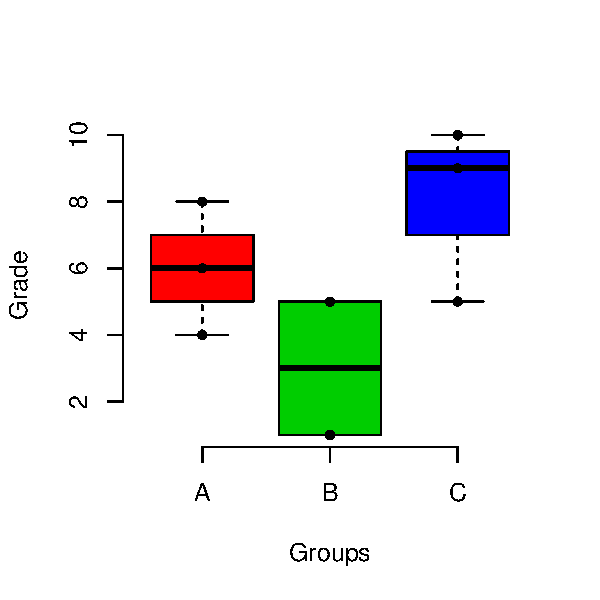
\includegraphics[width=.4\linewidth]{figures/plot-t2-plots-1} 
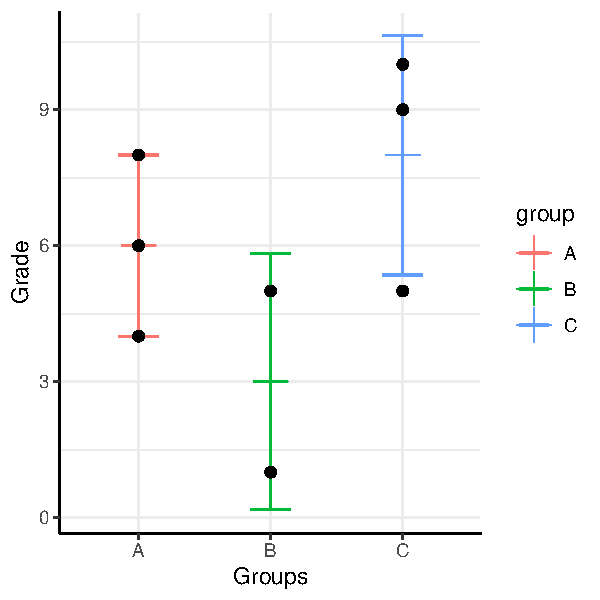
\includegraphics[width=.4\linewidth]{figures/plot-t2-plots-2} 

}



\end{knitrout}

Finaly, below we compute the ANOVA tests with our data using the function \verb+aov()+.

\begin{knitrout}
\definecolor{shadecolor}{rgb}{0.969, 0.969, 0.969}\color{fgcolor}\begin{kframe}
\begin{alltt}
\hlstd{fit} \hlkwb{<-} \hlkwd{aov}\hlstd{(grade} \hlopt{~} \hlstd{group,} \hlkwc{data} \hlstd{= X)}
\hlkwd{summary}\hlstd{(fit)}
\end{alltt}
\begin{verbatim}
##             Df Sum Sq Mean Sq F value Pr(>F)
## group        2     30      15     2.5  0.177
## Residuals    5     30       6
\end{verbatim}
\end{kframe}
\end{knitrout}

The F-statistic has a value of 2.5, which is above 1, which signifies some differences in group means. However the p-value is 0.177, which is not signigicant under the 5 \% significance level and therefore we cannot reject the null hypothesis of the group means being different.\\



Case (2):\\
Suppose that the first observation in the second group was actually 9, not 1. Then, the standard deviations are the same, but the sample means are 6, 7 and 8, rather than 6, 3 and 8. In this situation, we would expect the F-test statistic to be smaller. The main reason is that the differences in the group means are going to be smaller and therefore the nominator of the ratio, $S^2_{\text{between}}$ will be smaller and hence the whole ratio or F-statistic will be smaller. Since the F-value will be closer to 1 (or closer to the mean of F-distribution), the p-value will therefore also increase as observing statistics more extreme is more likely than before. \\

Case (3):\\
Suppose you have the same means as these data, but the sample standard deviations were 1.0, 1.8 and 1.6, instead of the actual 2.0, 2.8 and 2.6. In this situation, we would expect the F-test statistic to be larger. The main reason is that that the variation within each group have decreased and therefore the $S^2_{\text{within}}$ will decrease and since the denominator of the ratio will decrease, the whole F-test statistics will be larger. Since the F-statistics increased, the p-value will decrease (observing more extreme statistics is less likely). With such small variances, we could even expect the test to be significant at the 5\% significance level.\\

Case (4):\\
Suppose you have the same means and standard deviations as these data, but the sample size were 30, 20 and 30, instead of 3, 2 and 3. In this case, we would expect the F-test statistic to be larger. The main reason is the F-distribution with which we would be comparing our F-test statistic will be with 2 and 77 degrees of freedom. The groups variance still has the same number of degrees of freedom because the number of groups hasn't changed. However the residual variance now had 77 degrees of freedom compared to previously having only 5 degrees of freedom. Therefore, we would be dividing $S^2_{\text{within}}$ by 77, which would result in a signigicantly lower Mean Squared Residual compared to Mean Squared of Groups. Hence, the overall F-test statistics would significantly increase. With similar line of reasoning as before, as the F-statistics will be large, the p-value (probability of observing more extreme statistics) will be very low.\\

\section*{Task 3}

The compressive strength of concrete is being studied, and four different mixing techniques are being investigated. The following data have been collected. For each mixing technique, 4 compressive strength measurements (in pounds per square inch) have been recorded.\\

\begin{center}
\begin{tabular}{ l c c c c}
 \hline
 & \multicolumn{4}{c}{Compressive Strength} \\
 \hline
 Mixing & 1 & 2 & 3 & 4 \\
 \hline
 1 & 3129 & 3000 & 2865 & 2890 \\
 2 & 3200 & 3300 & 2975 & 3150 \\
 3 & 2800 & 2900 & 2985 & 3050 \\
 4 & 2600 & 2700 & 2600 & 2765 \\
 \hline
\end{tabular}
\end{center}

In this task we perform the same one-factor Analysis of Variance as in previous task. We load the data to R in following way and subsequently visualise it with same techniques as before. From the plots we can clearly see that some mixing techniques are quite different to others.

\begin{knitrout}
\definecolor{shadecolor}{rgb}{0.969, 0.969, 0.969}\color{fgcolor}\begin{kframe}
\begin{alltt}
\hlstd{X} \hlkwb{<-} \hlkwd{data.frame}\hlstd{(}\hlstr{"strength"}\hlstd{=}\hlkwd{c}\hlstd{(}\hlnum{3129}\hlstd{,}\hlnum{3000}\hlstd{,}\hlnum{2865}\hlstd{,}\hlnum{2890}\hlstd{,}
                             \hlnum{3200}\hlstd{,}\hlnum{3300}\hlstd{,}\hlnum{2975}\hlstd{,}\hlnum{3150}\hlstd{,}
                             \hlnum{2800}\hlstd{,}\hlnum{2900}\hlstd{,}\hlnum{2985}\hlstd{,}\hlnum{3050}\hlstd{,}
                             \hlnum{2600}\hlstd{,}\hlnum{2700}\hlstd{,}\hlnum{2600}\hlstd{,}\hlnum{2765}\hlstd{),}
                \hlstr{"mixing"}\hlstd{=}\hlkwd{rep}\hlstd{(}\hlkwd{c}\hlstd{(}\hlstr{"1"}\hlstd{,}\hlstr{"2"}\hlstd{,}\hlstr{"3"}\hlstd{,}\hlstr{"4"}\hlstd{),}\hlkwd{c}\hlstd{(}\hlnum{4}\hlstd{,}\hlnum{4}\hlstd{,}\hlnum{4}\hlstd{,}\hlnum{4}\hlstd{)) )}
\end{alltt}
\end{kframe}
\end{knitrout}


\begin{knitrout}
\definecolor{shadecolor}{rgb}{0.969, 0.969, 0.969}\color{fgcolor}

{\centering 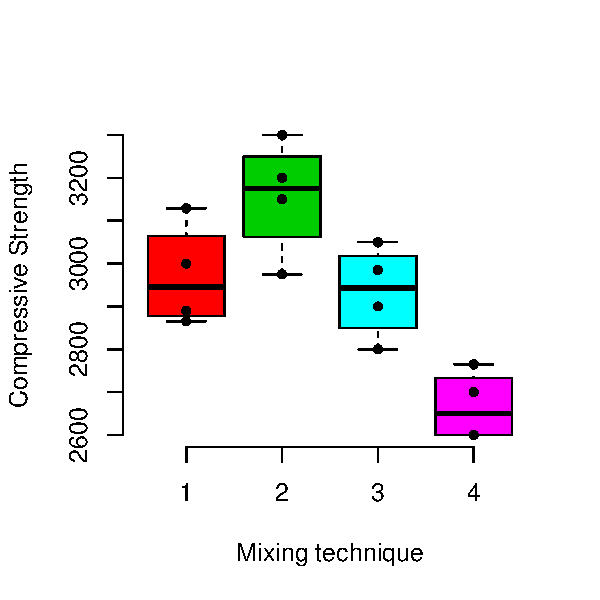
\includegraphics[width=.4\linewidth]{figures/plot-t3-plots-1} 
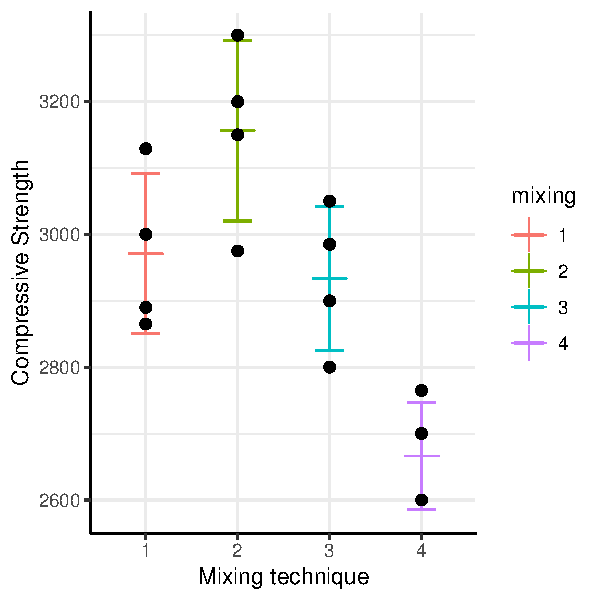
\includegraphics[width=.4\linewidth]{figures/plot-t3-plots-2} 

}



\end{knitrout}

Below, we perform the Analysis of Variance using again \verb+aov()+ function.\\

\begin{knitrout}
\definecolor{shadecolor}{rgb}{0.969, 0.969, 0.969}\color{fgcolor}\begin{kframe}
\begin{alltt}
\hlstd{fit} \hlkwb{<-} \hlkwd{aov}\hlstd{(strength} \hlopt{~} \hlstd{mixing,} \hlkwc{data} \hlstd{= X)}
\hlkwd{summary}\hlstd{(fit)}
\end{alltt}
\begin{verbatim}
##             Df Sum Sq Mean Sq F value   Pr(>F)    
## mixing       3 489740  163247   12.73 0.000489 ***
## Residuals   12 153908   12826                     
## ---
## Signif. codes:  0 '***' 0.001 '**' 0.01 '*' 0.05 '.' 0.1 ' ' 1
\end{verbatim}
\end{kframe}
\end{knitrout}

From the summary we can see that the F-statistics is 12.73, which is quite large for F-distribution with 3 and 12 degrees of freedom. This is also evident from the p-value being 0.0005, which is very small and we would therefore reject the null hypothesis that the group means are all the same. Therefore we can conclude there is some evidence that for at least one mixing technique, the compressive strength differs from others. But we cannot conclude which one differs. To yield this conclusion, we perform the multiple pairwise-comparison, to determine if the mean difference between specific pairs of group are statistically significant. \\

As the ANOVA test is significant, we can compute Tukey Honest Significant Differences for performing multiple pairwise-comparison between the means of groups. We use the function \verb+glht()+ [in \verb+multcomp+ package], where glht stands for general linear hypothesis tests.

\begin{knitrout}
\definecolor{shadecolor}{rgb}{0.969, 0.969, 0.969}\color{fgcolor}\begin{kframe}
\begin{alltt}
\hlkwd{library}\hlstd{(multcomp)}
\hlkwd{summary}\hlstd{(}\hlkwd{glht}\hlstd{(fit,} \hlkwc{linfct} \hlstd{=} \hlkwd{mcp}\hlstd{(}\hlkwc{mixing} \hlstd{=} \hlstr{"Tukey"}\hlstd{)))}
\end{alltt}
\begin{verbatim}
## 
## 	 Simultaneous Tests for General Linear Hypotheses
## 
## Multiple Comparisons of Means: Tukey Contrasts
## 
## 
## Fit: aov(formula = strength ~ mixing, data = X)
## 
## Linear Hypotheses:
##            Estimate Std. Error t value Pr(>|t|)    
## 2 - 1 == 0   185.25      80.08   2.313   0.1495    
## 3 - 1 == 0   -37.25      80.08  -0.465   0.9653    
## 4 - 1 == 0  -304.75      80.08  -3.806   0.0116 *  
## 3 - 2 == 0  -222.50      80.08  -2.778   0.0692 .  
## 4 - 2 == 0  -490.00      80.08  -6.119   <0.001 ***
## 4 - 3 == 0  -267.50      80.08  -3.340   0.0262 *  
## ---
## Signif. codes:  0 '***' 0.001 '**' 0.01 '*' 0.05 '.' 0.1 ' ' 1
## (Adjusted p values reported -- single-step method)
\end{verbatim}
\end{kframe}
\end{knitrout}

In the output we can see the individual comparisons between all groups with the p-value being adjusted for multiple testing such that in controls for the family-wise error rate. We can see that the largest differenence is between mixing techniques 4 and 2, where the estimate for the difference between those two is $-490$ with p-value being significant at all levels. The differences between mixing techniques 4 - 1 and 4 - 3 are also significant at level 0.05. With the estimated difference between both of them are negative, we can conclude that the mixing technique 4 has the smallest comptessive strength then all other mixing techniques. Hence, we would not recommend to use mixing technique 4 for concrete in practice.

\section*{Task 4}
Consider the data set munich.csv. The data set contains information on therent prices of apartments in Munich.  The variables in the data set are:

\begin{itemize}
\item rent:  net rent per month (in Euro)
\item area:  living area in square meters-yearc:
\item year of construction
\item location:  quality of location according to an expert assessment(0 = average location, 1 = good location, 2 = top location)
\end{itemize}

\begin{knitrout}
\definecolor{shadecolor}{rgb}{0.969, 0.969, 0.969}\color{fgcolor}\begin{kframe}
\begin{alltt}
\hlstd{munich} \hlkwb{<-} \hlkwd{read.csv}\hlstd{(}\hlstr{"munich.csv"}\hlstd{)}
\hlstd{munich}\hlopt{$}\hlstd{location} \hlkwb{<-} \hlkwd{factor}\hlstd{(munich}\hlopt{$}\hlstd{location)}
\end{alltt}
\end{kframe}
\end{knitrout}


\begin{knitrout}
\definecolor{shadecolor}{rgb}{0.969, 0.969, 0.969}\color{fgcolor}\begin{kframe}
\begin{alltt}
\hlkwd{par}\hlstd{(}\hlkwc{mfrow}\hlstd{=}\hlkwd{c}\hlstd{(}\hlnum{2}\hlstd{,}\hlnum{2}\hlstd{))}
\hlstd{year_agg} \hlkwb{<-} \hlkwd{aggregate}\hlstd{(munich}\hlopt{$}\hlstd{rent,} \hlkwd{list}\hlstd{(munich}\hlopt{$}\hlstd{yearc),}
                      \hlkwa{function}\hlstd{(}\hlkwc{x}\hlstd{)} \hlkwd{c}\hlstd{(}\hlkwc{mean}\hlstd{=}\hlkwd{mean}\hlstd{(x),} \hlkwc{sd}\hlstd{=}\hlkwd{sd}\hlstd{(x)))}
\hlkwd{plot}\hlstd{(year_agg}\hlopt{$}\hlstd{Group.1, year_agg}\hlopt{$}\hlstd{x[,}\hlstr{"mean"}\hlstd{],} \hlkwc{xlab}\hlstd{=}\hlstr{"year"}\hlstd{,}
     \hlkwc{ylab}\hlstd{=}\hlstr{"rent: mean +- 1 sd"}\hlstd{,} \hlkwc{ylim}\hlstd{=}\hlkwd{c}\hlstd{(}\hlnum{0}\hlstd{,} \hlnum{1300}\hlstd{))}
\hlkwd{segments}\hlstd{(year_agg}\hlopt{$}\hlstd{Group.1}\hlopt{-}\hlnum{0.25}\hlstd{, year_agg}\hlopt{$}\hlstd{x[,}\hlstr{"mean"}\hlstd{]}\hlopt{+}\hlstd{year_agg}\hlopt{$}\hlstd{x[,}\hlstr{"sd"}\hlstd{],}
          \hlstd{year_agg}\hlopt{$}\hlstd{Group.1}\hlopt{+}\hlnum{0.25}\hlstd{, year_agg}\hlopt{$}\hlstd{x[,}\hlstr{"mean"}\hlstd{]}\hlopt{+}\hlstd{year_agg}\hlopt{$}\hlstd{x[,}\hlstr{"sd"}\hlstd{],}\hlkwc{col}\hlstd{=}\hlstr{"grey"}\hlstd{)}
\hlkwd{segments}\hlstd{(year_agg}\hlopt{$}\hlstd{Group.1}\hlopt{-}\hlnum{0.25}\hlstd{, year_agg}\hlopt{$}\hlstd{x[,}\hlstr{"mean"}\hlstd{]}\hlopt{-}\hlstd{year_agg}\hlopt{$}\hlstd{x[,}\hlstr{"sd"}\hlstd{],}
          \hlstd{year_agg}\hlopt{$}\hlstd{Group.1}\hlopt{+}\hlnum{0.25}\hlstd{, year_agg}\hlopt{$}\hlstd{x[,}\hlstr{"mean"}\hlstd{]}\hlopt{-}\hlstd{year_agg}\hlopt{$}\hlstd{x[,}\hlstr{"sd"}\hlstd{],}\hlkwc{col}\hlstd{=}\hlstr{"grey"}\hlstd{)}
\hlkwd{segments}\hlstd{(year_agg}\hlopt{$}\hlstd{Group.1, year_agg}\hlopt{$}\hlstd{x[,}\hlstr{"mean"}\hlstd{]}\hlopt{+}\hlstd{year_agg}\hlopt{$}\hlstd{x[,}\hlstr{"sd"}\hlstd{],}
         \hlstd{year_agg}\hlopt{$}\hlstd{Group.1,year_agg}\hlopt{$}\hlstd{x[,}\hlstr{"mean"}\hlstd{]}\hlopt{-}\hlstd{year_agg}\hlopt{$}\hlstd{x[,}\hlstr{"sd"}\hlstd{],}\hlkwc{col}\hlstd{=}\hlstr{"grey"}\hlstd{)}


\hlkwd{plot}\hlstd{(rent}\hlopt{~}\hlstd{area,} \hlkwc{data}\hlstd{=munich)}
\hlkwd{plot}\hlstd{(rent}\hlopt{~}\hlstd{location,} \hlkwc{data}\hlstd{=munich)}
\end{alltt}
\end{kframe}

{\centering 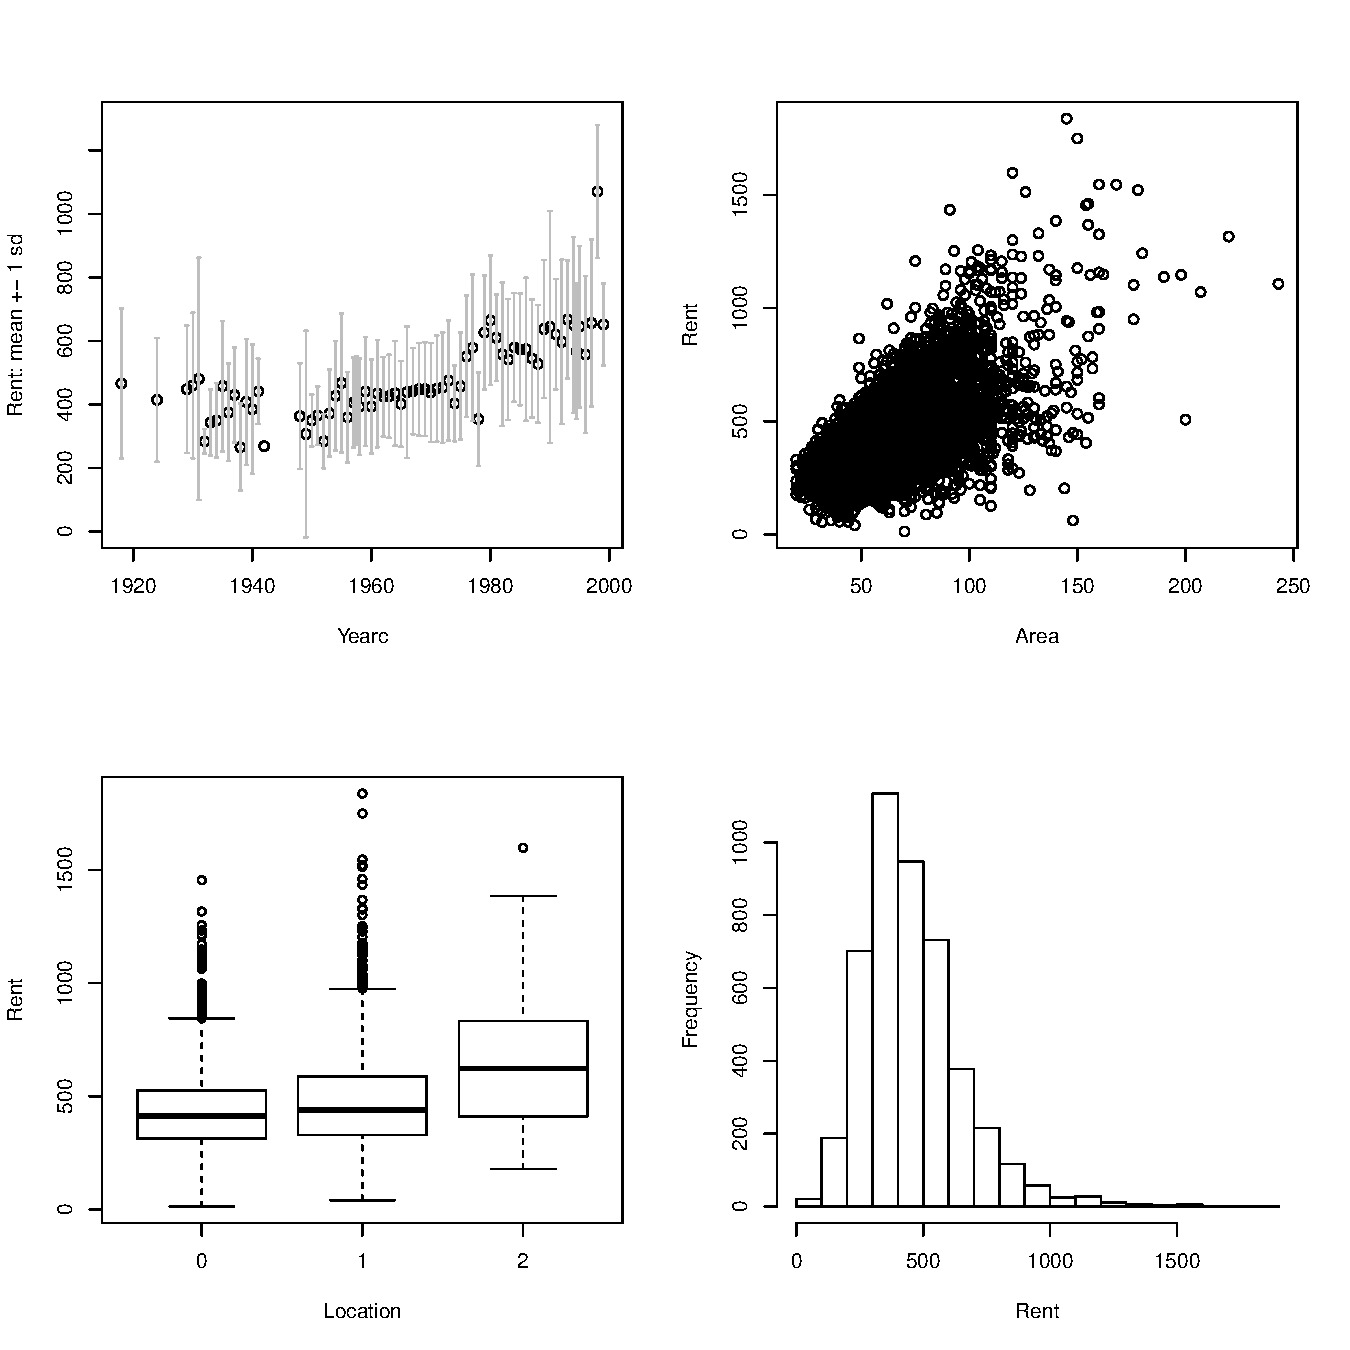
\includegraphics[width=\maxwidth]{figures/plot-t4-discuss-1} 

}



\end{knitrout}
From the above plots, we can already come to the reasonable conclusion that there is a relationship between rent and area, location, and year.

\begin{knitrout}
\definecolor{shadecolor}{rgb}{0.969, 0.969, 0.969}\color{fgcolor}\begin{kframe}
\begin{alltt}
\hlstd{f1} \hlkwb{<-} \hlkwd{lm}\hlstd{(rent}\hlopt{~}\hlstd{area}\hlopt{*}\hlstd{location} \hlopt{+} \hlstd{yearc,} \hlkwc{data}\hlstd{=munich)}
\hlkwd{par}\hlstd{(}\hlkwc{mfrow}\hlstd{=}\hlkwd{c}\hlstd{(}\hlnum{2}\hlstd{,}\hlnum{2}\hlstd{))}
\hlkwd{plot}\hlstd{(f1)}
\end{alltt}
\end{kframe}

{\centering 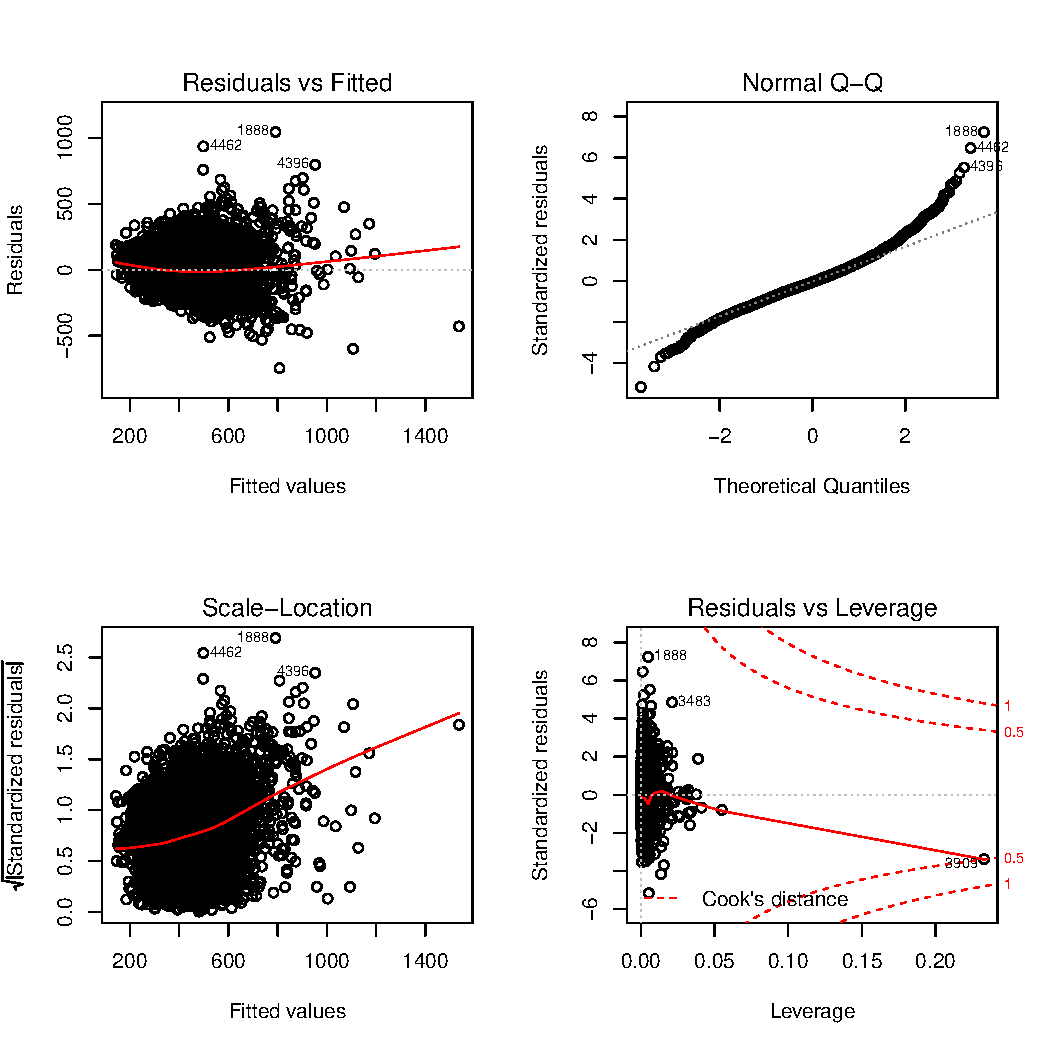
\includegraphics[width=\maxwidth]{figures/plot-t4-model-1} 

}



\end{knitrout}

From the 'Residuals vs Fitted' plot in the top left, we see that the assumption of zero-mean residuals holds (the trend line drifts away from zero as the fitted values go up, but this can be explained by the lack of data in that area of the plot). However, it could be argued that the variance of the errors increase with the fitted values, but this is quite hard to be sure of with this graph alone.\\

The 'Normal Q-Q' plot is perhaps a little concerning with the tails drifting away from the 'expected' line.\\

In the 'Scale-Location' graph, we again have evidence for heteroscedastic residuals, as the trend variance of residuals appears to get larger as the fitted values get larger (which we also observed in the first plot). However, it could be argued again that this major deviation of the trend line from the expected behaviour is due to a just a few datapoints. There is mounting evidence for heteroscedastic residuals, so perhaps a variable transformation is required.\\

Finally, in the 'Residuals vs Leverage' plot we can see that the majority of datapoints have low leverage and a relatively small Cook's distance. There is just one point, in row 3909, which has a high leverage as well as a high Cook's distance. This datapoint should be looked at in more detail as the analysis progresses beyond this initial phase.\\

\begin{knitrout}
\definecolor{shadecolor}{rgb}{0.969, 0.969, 0.969}\color{fgcolor}\begin{kframe}
\begin{alltt}
\hlkwd{summary}\hlstd{(f1)}
\end{alltt}
\begin{verbatim}
## 
## Call:
## lm(formula = rent ~ area * location + yearc, data = munich)
## 
## Residuals:
##     Min      1Q  Median      3Q     Max 
## -746.56  -86.86   -8.91   78.91 1046.26 
## 
## Coefficients:
##                  Estimate Std. Error t value Pr(>|t|)    
## (Intercept)    -5.356e+03  1.964e+02 -27.274  < 2e-16 ***
## area            4.732e+00  1.267e-01  37.344  < 2e-16 ***
## location1      -1.052e+00  1.302e+01  -0.081 0.935595    
## location2       1.219e+01  3.858e+01   0.316 0.752029    
## yearc           2.796e+00  9.971e-02  28.036  < 2e-16 ***
## area:location1  6.948e-01  1.802e-01   3.855 0.000117 ***
## area:location2  1.519e+00  4.449e-01   3.414 0.000646 ***
## ---
## Signif. codes:  0 '***' 0.001 '**' 0.01 '*' 0.05 '.' 0.1 ' ' 1
## 
## Residual standard error: 144.9 on 4564 degrees of freedom
## Multiple R-squared:  0.4575,	Adjusted R-squared:  0.4568 
## F-statistic: 641.5 on 6 and 4564 DF,  p-value: < 2.2e-16
\end{verbatim}
\end{kframe}
\end{knitrout}

The model results confirm our reasoning that there is a relationship between the three variables (area, location, and year) and rent. Both area and year have a very low p-value. Location has a high p-value which would at first glance suggest that it doesn't have a significant relationship with the rent value, however we can see that the interaction between location and area has a low p-value, so it is feasible that the 'information' given by location is captured in this interaction. It is good practice to leave this 'main effect' of location in the model still, as we will be including its interaction with area.

\begin{knitrout}
\definecolor{shadecolor}{rgb}{0.969, 0.969, 0.969}\color{fgcolor}\begin{kframe}
\begin{alltt}
\hlstd{f2} \hlkwb{<-} \hlkwd{lm}\hlstd{(rent}\hlopt{~}\hlstd{area,} \hlkwc{data}\hlstd{=munich)}
\hlkwd{summary}\hlstd{(f2)}
\end{alltt}
\begin{verbatim}
## 
## Call:
## lm(formula = rent ~ area, data = munich)
## 
## Residuals:
##     Min      1Q  Median      3Q     Max 
## -774.37  -99.85   -7.31   89.87 1016.36 
## 
## Coefficients:
##              Estimate Std. Error t value Pr(>|t|)    
## (Intercept) 135.63725    6.89211   19.68   <2e-16 ***
## area          4.73031    0.09541   49.58   <2e-16 ***
## ---
## Signif. codes:  0 '***' 0.001 '**' 0.01 '*' 0.05 '.' 0.1 ' ' 1
## 
## Residual standard error: 158.6 on 4569 degrees of freedom
## Multiple R-squared:  0.3498,	Adjusted R-squared:  0.3496 
## F-statistic:  2458 on 1 and 4569 DF,  p-value: < 2.2e-16
\end{verbatim}
\end{kframe}
\end{knitrout}



\begin{knitrout}
\definecolor{shadecolor}{rgb}{0.969, 0.969, 0.969}\color{fgcolor}\begin{kframe}
\begin{alltt}
\hlkwd{anova}\hlstd{(f2, f1)}
\end{alltt}
\begin{verbatim}
## Analysis of Variance Table
## 
## Model 1: rent ~ area
## Model 2: rent ~ area * location + yearc
##   Res.Df       RSS Df Sum of Sq      F    Pr(>F)    
## 1   4569 114891462                                  
## 2   4564  95857954  5  19033509 181.25 < 2.2e-16 ***
## ---
## Signif. codes:  0 '***' 0.001 '**' 0.01 '*' 0.05 '.' 0.1 ' ' 1
\end{verbatim}
\end{kframe}
\end{knitrout}

This analysis of variance shows that the larger model (i.e. including location, year, and the interaction between area and location) is significantly better than the smaller model of just including area. The Residual Sum of Squares is significantly lower, leading to a p-value that signifies a signicant result.


\end{document}
